\section{Overview}
ALIAS was developed using iterative approach. For each iteration a different approach for computing the extensions has been implemented. In order to verify and benchmark the approach, each iteration had allocated time for testing. Furthermore, the testing process can be divided into two separate processes: 
\begin{enumerate}
	\item Unit testing - number of tests has been created to verify the correctness of the proposed solution. Those tests are to verify if any change to the solution still produces correct output. 
	\item Benchmark testing - more extensive testing carried out at the end of each iteration. The purpose of the benchmark testing is to help evaluate the system. 
\end{enumerate}
However, the benchmark testing has been only performed on the preferred and stable extensions. This is due to complete extension being added to ALIAS in the final stages of the project.

\section{Testing Technique}
As described in section \ref{label:projectRequirements}, there are number of functional and non-functional requirements for ALIAS. One of the most critical set of requirements identified are the correctness of computed solution and the scalability. In order to verify those requirements the black-box testing technique was used. Black box testing as described by \citet{testing2} is "based on the analysis of the specification of a piece of software without reference to its internal working". Thus, in order to use the black-box testing technique, each implemented approach has been tested only when it was fully completed \citep{blackbox}.

\section{Data Sets}
In order to extensively test ALIAS, benchmark argumentation frameworks have been taken from the published sample argumentation frameworks from ICCMA 2017 \citep{iccmaResults}. The website provides 5 different sets of argumentation frameworks for all tasks involved in the competition and additional set for a Dung's Triathlon. As shown in section \ref{section:design}, selected argumentation frameworks have been classified into 5 categories: very easy, easy, medium, hard and too hard. 

Appendix \ref{appendix:benchmarkFiles} shows the full list of argumentation frameworks used including the number of arguments and attacks. Although, different set of frameworks have been used for testing preferred and complete extensions, and stable extension, it can be seen that size and complexity of the argumentation frameworks is varied. They include small framework including only 2 arguments and single attack to as much as six thousand arguments and over sixty thousand attacks in some cases. This is to help identify limits and possible issues with proposed solution. 

Additional benefit of using the benchmark frameworks from ICCMA 2017 competition is to be able to compare the results of ALIAS against the existing solutions. Furthermore, the benchmark testing can help identify the best solution and aid with improving the approach being used. With satisfactory results, ALIAS could take a part in the future competitions.

\section{Unit testing}
Unit tests played important role during the development of each approach for ALIAS. Every change to the proposed solution has been tested and verified by using small number of argumentation frameworks. Each framework has been created and tested using other systems like Pyglaf and ArgSemSAT to ensure the outputted extensions are correct. 

Although unit testing does not help with evaluating the overall performance of ALIAS, it played critical role during the development of ALIAS. Before each change to the solution has been checked in to source control, unit tests had to be executed to ensure they still pass. 

\section{Performance}
As \citet{performanceTesting1} points out, performance requirements play a key role in determining the usability and quality of many systems. In case of ALIAS the biggest concern in terms of performance is scalability. Argumentation frameworks used for unit testing were small in comparison to frameworks used in real world application or competitions like ICCMA. Thus, to correctly evaluate the performance and abilities of ALIAS, benchmark argumentation frameworks from appendix \ref{appendix:benchmarkFiles} have been used.

In order to test the scalability and performance, each implemented solution has been put through extensive testing. For each extension implemented within the proposed solutions, tests have been executed using the appropriate argumentation frameworks from appendix \ref{appendix:benchmarkFiles}. Each test run has been executed on the same machine with following specifications:

\begin{itemize}
	\item Processor: Intel Core I5-6200U @ 2.30 GHz
	\item GPU: Nvidia GeForce 940MX
	\item RAM: 8GB
	\item OS: Linux based
\end{itemize}

Using the same specifications for each test run allows for the test results to be easily comparable. Furthermore, since ICCMA 2017 competition has been ran on a different machines, Pyglaf \citep{pyglaf} and ArgMatSAT \citep{argmatSat} have been put through the same benchmark testing using the same machine. Those results were used to compare and evaluate the performance of ALIAS to the most successful solvers submitted to ICCMA 2017.

During testing, CPU time has been limited per each argumentation framework to 20 minutes. This is to prevent the solver from computing the extensions indefinitely, especially on larger and more complex argumentation frameworks. The time required to read and parse files was not included in the specified time limit and it was used purely for computing all extensions. 

There were four separate proposed solution for computing abstract argumentation. Three of them were using same method of computing the maximal conflict free set, but using different data structures to overcome certain issues and limitations as described in section \ref{section:maxConflictFreeSet}. The final approach is using SAT solver to enumerate possible solutions (see section \ref{section:satSolver}). Each approach was generating a number of possible solutions, which were then verified using matrix approach for preferred extension and set inclusion for stable extension as shown in sections \ref{section:preferredExtension} and \ref{section:stableExtension} respectively. 

\subsection{Stable Extension results} \label{section:stableExtensionResults}
Figure \ref{fig:stableFinalResults} shows the execution times of all four approaches: sets, PyTables, parallel dictionaries and SAT solver for computing all Stable Extension on the set of argumentation frameworks specified in appendix \ref{appendix:benchmarkFiles}. The chart only shows the timings for first 44 frameworks, as all the approaches timed out for the few final frameworks.

As it can be seen in chart \ref{fig:stableFinalResults}, certain data points are missing for some of the approaches. This is due to the solver reaching a 20 minutes time limit without providing the solution. Hence, no time has been recorded for given argumentation framework.

Based on the results shown in figure \ref{fig:stableFinalResults}, approach using parallel dictionaries had the highest number of computed extensions. Furthermore, it has the shortest execution time for majority of the time across all approaches, with exception for eight of them, where SAT solver approach considerably outperformed it. The execution time of dictionaries approach closely correspond to the approach using sets. Although sets operation are highly optimized in Python, it still did not outperform the implementation using dictionaries.

The worst performing solution is PyTables approach to computing and storing the Maximal Conflict Free Sets. This approach only computed the extensions for first five argumentation frameworks, which had the lowest number of arguments and relations between them. Those results are due to dynamically creating the sets iterating through all attacks within the argumentation framework as shown in section \ref{section:maxConflictFreeSet}. Since PyTables stores data on the hard drive, the read/write access creates high latency in terms of getting and storing values. This in turn has an impact on the overall performance causing ALIAS to reach the time out limit for the remaining argumentation frameworks.

\afterpage{
\begin{landscape}
	\begin{figure}
		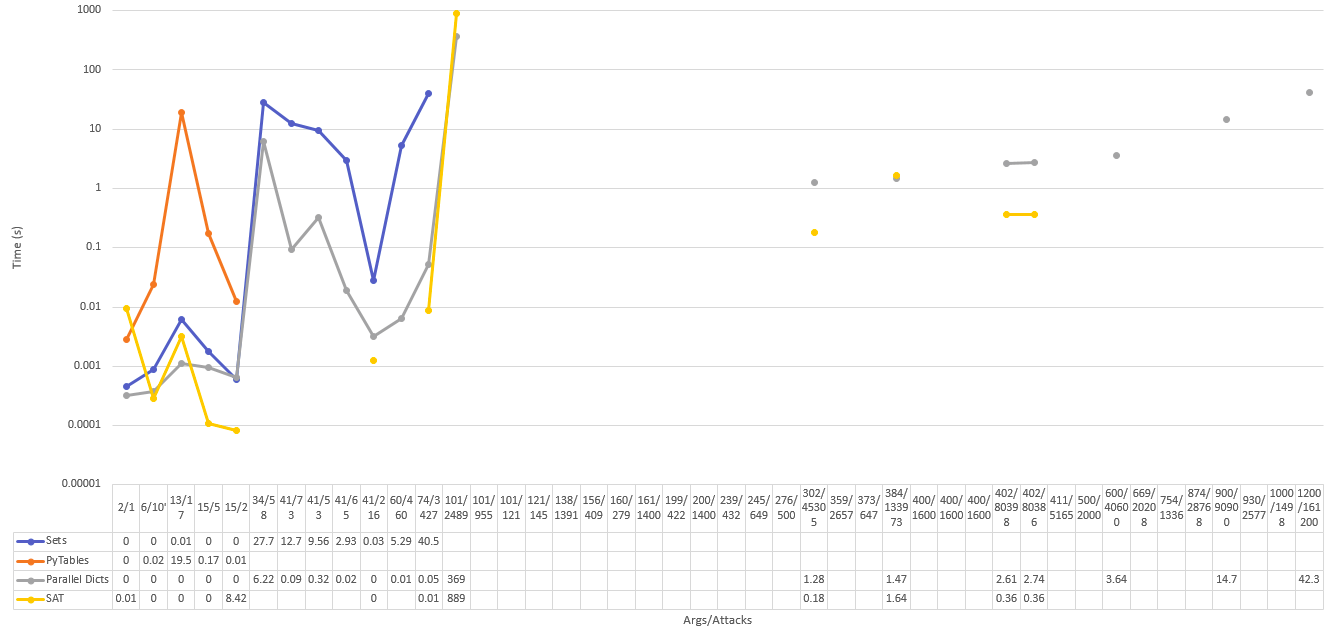
\includegraphics[width=21cm]{stableResults2}
		\caption{Timings of 4 approaches computing Stable Extension}
		\label{fig:stableFinalResults}
	\end{figure}
\end{landscape}
}

\subsection{Preferred Extension results} \label{section:preferredExtensionResults}
Results of timed execution of computing Preferred extension in all approaches implemented can be seen in figure \ref{fig:preferredFinalResults}. The chart shows results for the first 34 argumentation frameworks from benchmark files for preferred extension (see appendix \ref{appendix:benchmarkFiles}). Remaining 16 frameworks are not included due to all solution timing out.

Similarly to the stable extension results, two approaches are dominating: direct approach using parallel dictionaries and reduction based approach using SAT solver. Both of the approaches produced results for most of the argumentation frameworks. Furthermore, dictionaries approach outperformed the SAT based approach in majority of the results by being considerably faster.


Again, using data store from PyTables turned to be the least effective way. This solution managed to produce results only for the first four argumentation frameworks. Additionally, the approach using sets data structure correlate to approach using dictionaries. However, as it was the case with stable extension, it only managed to compute results for first few argumentation frameworks. Due to memory usage problem, this solution timed out for the remaining frameworks.

\afterpage{
\begin{landscape}
	\begin{figure}[h]
		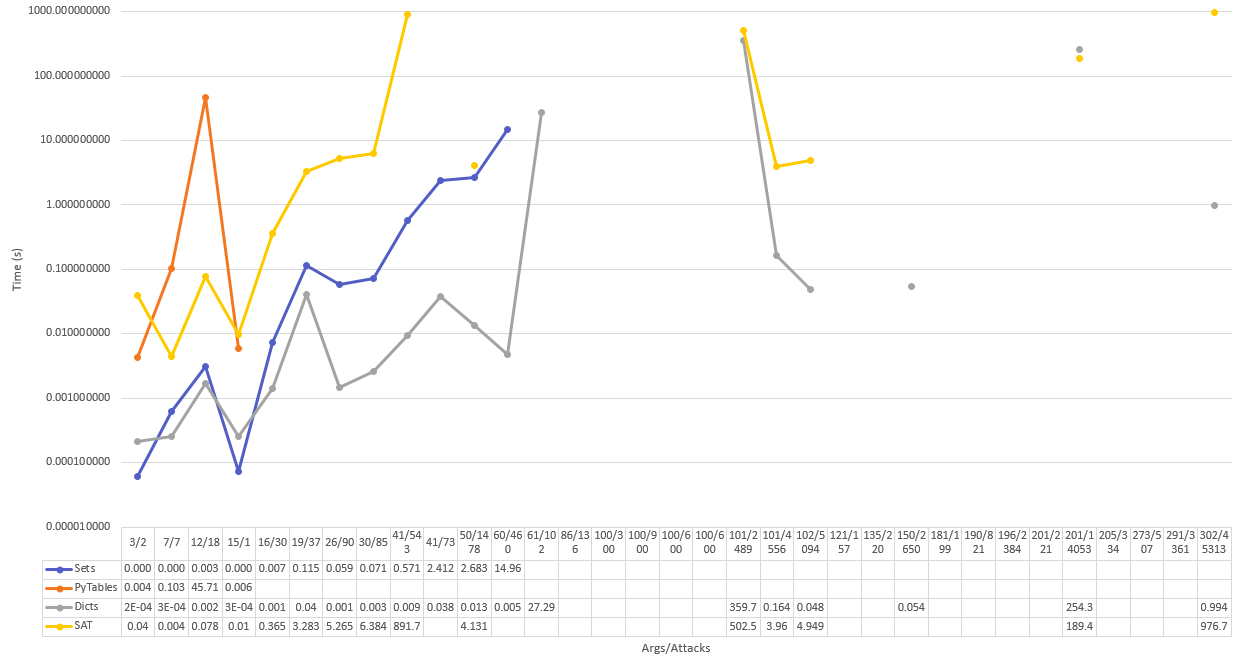
\includegraphics[width=21cm]{preferredResults2}
		\caption{Timings of 4 approaches computing Preferred Extension}
		\label{fig:preferredFinalResults}
	\end{figure}
\end{landscape}
}

\section{Correctness}
Correctness of the computed semantic is the critical functionality of the successful solver. However, it has introduced the challenge of finding the best way to verify the produced solution. There are number of formal approaches that could be applied to solver in order to confirm it provides the correct answer. For example, formal method called Z, "formal specification methodology that can dramatically improve the way software systems are modeled and implemented" \citep{potter1996introduction}, could be used to model the application and provide the proof of correctness. Although defining the approach and modeling the system could provide the guarantee for correctness of the application, this is outside the scope of this project. 

% Please add the following required packages to your document preamble:
% \usepackage{longtable}
% Note: It may be necessary to compile the document several times to get a multi-page table to line up properly
\begin{table}[!h]
	\centering
	\caption{Comparison of results for complete, stable and preferred extensions}
	\label{table:prefCorrectnes}
	\begin{tabular}{|c|c|c|c|}
		AF	& Complete & Stable & Preferred \\ \hline \hline
		%
		1 &   \cellcolor{green}\Checkmark    &   \cellcolor{green}\Checkmark     &    \cellcolor{green}\Checkmark        \\ \hline
		2 &   \cellcolor{green}\Checkmark    &   \cellcolor{green}\Checkmark     &    \cellcolor{green}\Checkmark        \\\hline
		3 &   \cellcolor{green}\Checkmark    &   \cellcolor{green}\Checkmark     &    \cellcolor{green}\Checkmark        \\\hline
		4 &   \cellcolor{green}\Checkmark    &   \cellcolor{green}\Checkmark     &    \cellcolor{green}\Checkmark        \\\hline
		5 &   \cellcolor{green}\Checkmark    &   \cellcolor{green}\Checkmark     &    \cellcolor{green}\Checkmark        \\\hline
		6 &   \cellcolor{green}\Checkmark    &   \cellcolor{green}\Checkmark     &    \cellcolor{green}\Checkmark        \\\hline
		7 &   \cellcolor{green}\Checkmark    &   \cellcolor{green}\Checkmark     &    \cellcolor{green}\Checkmark        \\\hline
		8 &   \cellcolor{green}\Checkmark    &   \cellcolor{green}\Checkmark     &    \cellcolor{green}\Checkmark        \\\hline
		9 &   \cellcolor{green}\Checkmark    &    \cellcolor{green}\Checkmark    &       \cellcolor{red}\cross     \\\hline
		10 &   \cellcolor{red}\cross    &    \cellcolor{green}\Checkmark    &       \cellcolor{green}\Checkmark \\  \hline
	\end{tabular}
\end{table}

Thus, In order to verify correctness of ALIAS, same argumentation frameworks from appendix \ref{appendix:benchmarkFiles} have been used as for the performance testing. Outputs of SAT based approach have been compared to the results of two winning solvers: Pyglaf \citep{pyglaf} and ArgSem-SAT \citep{argsemsat}. Although this does not guarantee the correct results, those solvers were the two highest scoring solvers in the competition. Thus, if their results are equal, the probability of answer being incorrect is low.

Table \ref{table:prefCorrectnes} shows the results of comparisons of extension results for the first 10 argumentation frameworks from benchmark frameworks (see appendix \ref{appendix:benchmarkFiles}). As mentioned above, output from ALIAS has been compared to output from Pyglaf and ArgSem-SAT. Although the correctness tests have been performed on the small set of argumentation framework, it can be seen that for complete and preferred extensions there were one set for each semantic, where the output differ from the leading solvers. On the other hand, no issues were found for stable semantic. Based on those results, following metric for ALIAS can be specified:
\begin{itemize}
	\item Complete - correctness 90\%
	\item Stable - correctness 100\%
	\item Preferred - correctness 90\%
\end{itemize}


\section{Web UI Test Cases} \label{section:testCases}
In order to test the functionality of ALIAS Web User Interface, number of test cases has been created and executed. Those test cases correspond to each \textit{Must} and \textit{Should Have} requirement from the Web UI requirements. Tables \ref{table:testcase1} to \ref{table:testcase8} show the scenarios tested and results of each test.

% Please add the following required packages to your document preamble:
% \usepackage{longtable}
% Note: It may be necessary to compile the document several times to get a multi-page table to line up properly
\renewcommand{\arraystretch}{1.5}
\begin{longtable}[c]{p{0.05\textwidth}|p{0.2\textwidth}|p{0.2\textwidth}|p{0.4\textwidth}|p{0.05\textwidth}}
	\caption{Web UI - Test Case 1}
	\label{table:testcase1}
	\\
	\hline
	\multicolumn{2}{p{0.3\textwidth}}{\textbf{Scenario}} & \multicolumn{3}{p{0.6\textwidth}}{User should be able to load predefined example argumentation frameworks} \\ 
	\hline
	\endfirsthead
	%
	\endhead
	%
	\multicolumn{2}{p{0.3\textwidth}}{\textbf{Related Requirements}} & \multicolumn{3}{p{0.6\textwidth}}{WebUI.1} \\ 
	\hline
	\multicolumn{2}{p{0.3\textwidth}}{\textbf{Priority}} & \multicolumn{3}{p{0.6\textwidth}}{Critical} \\ 
	\hline
	\multicolumn{2}{p{0.3\textwidth}}{\textbf{Actor}} & \multicolumn{3}{p{0.6\textwidth}}{Web User} \\ 
	\hline
	\multicolumn{2}{p{0.3\textwidth}}{\textbf{Precondition}} & \multicolumn{3}{p{0.6\textwidth}}{Web server is running and example argumentation frameworks are provided} \\ 
	\hline
	\multicolumn{2}{p{0.3\textwidth}}{\textbf{Postcondition}} & \multicolumn{3}{p{0.6\textwidth}}{Graph of an example argumentation framework is displayed on the page} \\ 
	\hline
	\multicolumn{5}{c}{\cellcolor{grey}\textbf{TEST EXECUTION}} \\ 
	\hline
	\textbf{ID} & \multicolumn{2}{|p{0.4\textwidth}|}{\textbf{User Action}} & \textbf{System Response} & \textbf{P/F} \\ 
	\hline
	1 & \multicolumn{2}{|p{0.4\textwidth}|}{User clicks on the 'Examples' drop down list in the toolbar} & List of predefined example argumentation frameworks is displayed & P \\ 
	\hline
	2 & \multicolumn{2}{|p{0.4\textwidth}|}{User clicks on an item from 'Examples' drop down list} & Selected example argumentation framework is displayed in the graph format & P \\ \hline 
\end{longtable}


\begin{longtable}[c]{p{0.05\textwidth}|p{0.2\textwidth}|p{0.2\textwidth}|p{0.4\textwidth}|p{0.05\textwidth}}
	\caption{Web UI - Test Case 2}
	\label{table:testcase2} \\
	\hline
	\multicolumn{2}{p{0.3\textwidth}}{\textbf{Scenario}} & \multicolumn{3}{p{0.6\textwidth}}{User should be able to discard existing and create new argumentation framework} \\ 
	\hline
	\endfirsthead
	%
	\endhead
	%
	\multicolumn{2}{p{0.3\textwidth}}{\textbf{Related Requirements}} & \multicolumn{3}{p{0.6\textwidth}}{WebUI.2} \\ 
	\hline
	\multicolumn{2}{p{0.3\textwidth}}{\textbf{Priority}} & \multicolumn{3}{p{0.6\textwidth}}{Critical} \\ 
	\hline
	\multicolumn{2}{p{0.3\textwidth}}{\textbf{Actor}} & \multicolumn{3}{p{0.6\textwidth}}{Web User} \\ 
	\hline
	\multicolumn{2}{p{0.3\textwidth}}{\textbf{Precondition}} & \multicolumn{3}{p{0.6\textwidth}}{Web server is running and argumentation framework is displayed on the page} \\ 
	\hline
	\multicolumn{2}{p{0.3\textwidth}}{\textbf{Postcondition}} & \multicolumn{3}{p{0.6\textwidth}}{Existing argumentation framework is discarded} \\ 
	\hline
	\multicolumn{5}{c}{\cellcolor{grey}\textbf{TEST EXECUTION}} \\ 
	\hline
	\textbf{ID} & \multicolumn{2}{|p{0.4\textwidth}|}{\textbf{User Action}} & \textbf{System Response} & \textbf{P/F} \\ 
	\hline
	1 & \multicolumn{2}{|p{0.4\textwidth}|}{User clicks 'New Framework' button from the toolbar} & Existing framework is discarded and graph is no longer displayed for that framework & P \\ 
	\hline
\end{longtable}

\begin{longtable}[c]{p{0.05\textwidth}|p{0.2\textwidth}|p{0.2\textwidth}|p{0.4\textwidth}|p{0.05\textwidth}}
	\caption{Web UI - Test Case 3}
	\label{table:testcase3} \\
	\hline
	\multicolumn{2}{p{0.3\textwidth}}{\textbf{Scenario}} & \multicolumn{3}{p{0.6\textwidth}}{User should be able to add arguments to argumentation framework} \\ 
	\hline
	\endfirsthead
	%
	\endhead
	%
	\multicolumn{2}{p{0.3\textwidth}}{\textbf{Related Requirements}} & \multicolumn{3}{p{0.6\textwidth}}{WebUI.3} \\ 
	\hline
	\multicolumn{2}{p{0.3\textwidth}}{\textbf{Priority}} & \multicolumn{3}{p{0.6\textwidth}}{Critical} \\ 
	\hline
	\multicolumn{2}{p{0.3\textwidth}}{\textbf{Actor}} & \multicolumn{3}{p{0.6\textwidth}}{Web User} \\ 
	\hline
	\multicolumn{2}{p{0.3\textwidth}}{\textbf{Precondition}} & \multicolumn{3}{p{0.6\textwidth}}{Web server is running} \\ 
	\hline
	\multicolumn{2}{p{0.3\textwidth}}{\textbf{Postcondition}} & \multicolumn{3}{p{0.6\textwidth}}{New argument is added to argumentation framework} \\ 
	\hline
	\multicolumn{5}{c}{\cellcolor{grey}\textbf{TEST EXECUTION}} \\ 
	\hline
	\textbf{ID} & \multicolumn{2}{|p{0.4\textwidth}|}{\textbf{User Action}} & \textbf{System Response} & \textbf{P/F} \\ 
	\hline
	1 & \multicolumn{2}{|p{0.4\textwidth}|}{User clicks 'New Framework' button from the toolbar} & Any existing framework is discarded and graph is no longer displayed for that framework & P \\ 
	\hline
	2 & \multicolumn{2}{|p{0.4\textwidth}|}{User clicks 'Add Argument' button from the toolbar} & Modal window is shown prompting user to enter name for the new argument & P \\ 
	\hline
	3 & \multicolumn{2}{|p{0.4\textwidth}|}{User enters a name for the new argument} & New name is displayed in the field & P \\ 
	\hline
	4 & \multicolumn{2}{|p{0.4\textwidth}|}{User clicks 'Add' button on the modal form} & Modal form disappears and argument with specified name is added to the argumentation framework and is displayed as a graph on the page & P \\ 
	\hline
\end{longtable}

\begin{longtable}[c]{p{0.05\textwidth}|p{0.2\textwidth}|p{0.2\textwidth}|p{0.4\textwidth}|p{0.05\textwidth}}
	\caption{Web UI - Test Case 4}
	\label{table:testcase4} \\
	\hline
	\multicolumn{2}{p{0.3\textwidth}}{\textbf{Scenario}} & \multicolumn{3}{p{0.6\textwidth}}{User should be able to add attacks to argumentation framework} \\ 
	\hline
	\endfirsthead
	%
	\endhead
	%
	\multicolumn{2}{p{0.3\textwidth}}{\textbf{Related Requirements}} & \multicolumn{3}{p{0.6\textwidth}}{WebUI.4} \\ 
	\hline
	\multicolumn{2}{p{0.3\textwidth}}{\textbf{Priority}} & \multicolumn{3}{p{0.6\textwidth}}{Critical} \\ 
	\hline
	\multicolumn{2}{p{0.3\textwidth}}{\textbf{Actor}} & \multicolumn{3}{p{0.6\textwidth}}{Web User} \\ 
	\hline
	\multicolumn{2}{p{0.3\textwidth}}{\textbf{Precondition}} & \multicolumn{3}{p{0.6\textwidth}}{Web server is running} \\ 
	\hline
	\multicolumn{2}{p{0.3\textwidth}}{\textbf{Postcondition}} & \multicolumn{3}{p{0.6\textwidth}}{New attack is added to argumentation framework} \\ 
	\hline
	\multicolumn{5}{c}{\cellcolor{grey}\textbf{TEST EXECUTION}} \\ 
	\hline
	\textbf{ID} & \multicolumn{2}{|p{0.4\textwidth}|}{\textbf{User Action}} & \textbf{System Response} & \textbf{P/F} \\ 
	\hline
	1 & \multicolumn{2}{|p{0.4\textwidth}|}{User clicks 'New Framework' button from the toolbar} & Any existing framework is discarded and graph is no longer displayed for that framework & P \\ 
	\hline
	2 & \multicolumn{2}{|p{0.4\textwidth}|}{User clicks 'Add Attack' button from the toolbar} & Modal window is shown prompting user to enter name of the attacking and attacked argument & P \\ 
	\hline
	3 & \multicolumn{2}{|p{0.4\textwidth}|}{User enters a name for the attacking argument} & Attacker name is displayed in the field & P \\ 
	\hline
	4 & \multicolumn{2}{|p{0.4\textwidth}|}{User enters a name for the attacked argument} & Attacked name is displayed in the field & P \\ 
	\hline
	5 & \multicolumn{2}{|p{0.4\textwidth}|}{User clicks 'Add' button on the modal form} & Modal form disappears and two argument: attacker and attacked, are added to the argumentation framework and displayed on the page and correct relation from attacker to attacked is shown on the graph & P \\ 
	\hline
\end{longtable}


\begin{longtable}[c]{p{0.05\textwidth}|p{0.2\textwidth}|p{0.2\textwidth}|p{0.4\textwidth}|p{0.05\textwidth}}
	\caption{Web UI - Test Case 5}
	\label{table:testcase5} \\
	\hline
	\multicolumn{2}{p{0.3\textwidth}}{\textbf{Scenario}} & \multicolumn{3}{p{0.6\textwidth}}{User should be able to view Complete Extensions of given argumentation framework} \\ 
	\hline
	\endfirsthead
	%
	\endhead
	%
	\multicolumn{2}{p{0.3\textwidth}}{\textbf{Related Requirements}} & \multicolumn{3}{p{0.6\textwidth}}{WebUI.11} \\ 
	\hline
	\multicolumn{2}{p{0.3\textwidth}}{\textbf{Priority}} & \multicolumn{3}{p{0.6\textwidth}}{Critical} \\ 
	\hline
	\multicolumn{2}{p{0.3\textwidth}}{\textbf{Actor}} & \multicolumn{3}{p{0.6\textwidth}}{Web User} \\ 
	\hline
	\multicolumn{2}{p{0.3\textwidth}}{\textbf{Precondition}} & \multicolumn{3}{p{0.6\textwidth}}{Web server is running and argumentation framework is loaded into the system and displayed as a graph} \\ 
	\hline
	\multicolumn{2}{p{0.3\textwidth}}{\textbf{Postcondition}} & \multicolumn{3}{p{0.6\textwidth}}{Complete extension is computed and the result shown. User can view each individual solution} \\ 
	\hline
	\multicolumn{5}{c}{\cellcolor{grey}\textbf{TEST EXECUTION}} \\ 
	\hline
	\textbf{ID} & \multicolumn{2}{|p{0.4\textwidth}|}{\textbf{User Action}} & \textbf{System Response} & \textbf{P/F} \\ 
	\hline
	1 & \multicolumn{2}{|p{0.4\textwidth}|}{User clicks 'Extensions' drop down link in the toolbar} & List of all available extensions is displayed & P \\ 
	\hline
	2 & \multicolumn{2}{|p{0.4\textwidth}|}{User clicks 'Complete' from the drop down list} & All Complete extensions for the given argumentation framework are computed and displayed as a list on the right hand side of the page & P \\ 
	\hline
	3 & \multicolumn{2}{|p{0.4\textwidth}|}{User clicks one of the solution from the list of all Complete extensions} & All arguments from the selected solutions are highlighted in green and label is displayed in white bold text & P \\ 
	\hline
	4 & \multicolumn{2}{|p{0.4\textwidth}|}{User clicks another solution from the list of all Complete extensions with different argument} & Highlighted styling is removed from any already highlighted arguments and all arguments from the selected solutions are highlighted in green and label is displayed in white bold text & P \\ 
	\hline
\end{longtable}

\begin{longtable}[c]{p{0.05\textwidth}|p{0.2\textwidth}|p{0.2\textwidth}|p{0.4\textwidth}|p{0.05\textwidth}}
	\caption{Web UI - Test Case 6}
	\label{table:testcase6} \\
	\hline
	\multicolumn{2}{p{0.3\textwidth}}{\textbf{Scenario}} & \multicolumn{3}{p{0.6\textwidth}}{User should be able to view Stable Extensions of given argumentation framework} \\ 
	\hline
	\endfirsthead
	%
	\endhead
	%
	\multicolumn{2}{p{0.3\textwidth}}{\textbf{Related Requirements}} & \multicolumn{3}{p{0.6\textwidth}}{WebUI.14} \\ 
	\hline
	\multicolumn{2}{p{0.3\textwidth}}{\textbf{Priority}} & \multicolumn{3}{p{0.6\textwidth}}{Critical} \\ 
	\hline
	\multicolumn{2}{p{0.3\textwidth}}{\textbf{Actor}} & \multicolumn{3}{p{0.6\textwidth}}{Web User} \\ 
	\hline
	\multicolumn{2}{p{0.3\textwidth}}{\textbf{Precondition}} & \multicolumn{3}{p{0.6\textwidth}}{Web server is running and argumentation framework is loaded into the system and displayed as a graph} \\ 
	\hline
	\multicolumn{2}{p{0.3\textwidth}}{\textbf{Postcondition}} & \multicolumn{3}{p{0.6\textwidth}}{Stable extension is computed and the result shown. User can view each individual solution} \\ 
	\hline
	\multicolumn{5}{c}{\cellcolor{grey}\textbf{TEST EXECUTION}} \\ 
	\hline
	\textbf{ID} & \multicolumn{2}{|p{0.4\textwidth}|}{\textbf{User Action}} & \textbf{System Response} & \textbf{P/F} \\ 
	\hline
	1 & \multicolumn{2}{|p{0.4\textwidth}|}{User clicks 'Extensions' drop down link in the toolbar} & List of all available extensions is displayed & P \\ 
	\hline
	2 & \multicolumn{2}{|p{0.4\textwidth}|}{User clicks 'Stable' from the drop down list} & All Stable extensions for the given argumentation framework are computed and displayed as a list on the right hand side of the page & P \\ 
	\hline
	3 & \multicolumn{2}{|p{0.4\textwidth}|}{User clicks one of the solution from the list of all Stable extensions} & All arguments from the selected solutions are highlighted in green and label is displayed in white bold text & P \\ 
	\hline
	4 & \multicolumn{2}{|p{0.4\textwidth}|}{User clicks another solution from the list of all Stable extensions with different argument} & Highlighted styling is removed from any already highlighted arguments and all arguments from the selected solutions are highlighted in green and label is displayed in white bold text & P \\ 
	\hline
\end{longtable}

\begin{longtable}[c]{p{0.05\textwidth}|p{0.2\textwidth}|p{0.2\textwidth}|p{0.4\textwidth}|p{0.05\textwidth}}
	\caption{Web UI - Test Case 7}
	\label{table:testcase7} \\
	\hline
	\multicolumn{2}{p{0.3\textwidth}}{\textbf{Scenario}} & \multicolumn{3}{p{0.6\textwidth}}{User should be able to view Preferred Extensions of given argumentation framework} \\ 
	\hline
	\endfirsthead
	%
	\endhead
	%
	\multicolumn{2}{p{0.3\textwidth}}{\textbf{Related Requirements}} & \multicolumn{3}{p{0.6\textwidth}}{WebUI.17} \\ 
	\hline
	\multicolumn{2}{p{0.3\textwidth}}{\textbf{Priority}} & \multicolumn{3}{p{0.6\textwidth}}{Critical} \\ 
	\hline
	\multicolumn{2}{p{0.3\textwidth}}{\textbf{Actor}} & \multicolumn{3}{p{0.6\textwidth}}{Web User} \\ 
	\hline
	\multicolumn{2}{p{0.3\textwidth}}{\textbf{Precondition}} & \multicolumn{3}{p{0.6\textwidth}}{Web server is running and argumentation framework is loaded into the system and displayed as a graph} \\ 
	\hline
	\multicolumn{2}{p{0.3\textwidth}}{\textbf{Postcondition}} & \multicolumn{3}{p{0.6\textwidth}}{Preferred extension is computed and the result shown. User can view each individual solution} \\ 
	\hline
	\multicolumn{5}{c}{\cellcolor{grey}\textbf{TEST EXECUTION}} \\ 
	\hline
	\textbf{ID} & \multicolumn{2}{|p{0.4\textwidth}|}{\textbf{User Action}} & \textbf{System Response} & \textbf{P/F} \\ 
	\hline
	1 & \multicolumn{2}{|p{0.4\textwidth}|}{User clicks 'Extensions' drop down link in the toolbar} & List of all available extensions is displayed & P \\ 
	\hline
	2 & \multicolumn{2}{|p{0.4\textwidth}|}{User clicks 'Preferred' from the drop down list} & All Preferred extensions for the given argumentation framework are computed and displayed as a list on the right hand side of the page & P \\ 
	\hline
	3 & \multicolumn{2}{|p{0.4\textwidth}|}{User clicks one of the solution from the list of all Preferred extensions} & All arguments from the selected solutions are highlighted in green and label is displayed in white bold text & P \\ 
	\hline
	4 & \multicolumn{2}{|p{0.4\textwidth}|}{User clicks another solution from the list of all Preferred extensions with different argument} & Highlighted styling is removed from any already highlighted arguments and all arguments from the selected solutions are highlighted in green and label is displayed in white bold text & P \\ 
	\hline
\end{longtable}

\begin{longtable}[c]{p{0.05\textwidth}|p{0.2\textwidth}|p{0.2\textwidth}|p{0.4\textwidth}|p{0.05\textwidth}}
	\caption{Web UI - Test Case 8}
	\label{table:testcase8} \\
	\hline
	\multicolumn{2}{p{0.3\textwidth}}{\textbf{Scenario}} & \multicolumn{3}{p{0.6\textwidth}}{User should be able upload argumentation framework in tgf format} \\ 
	\hline
	\endfirsthead
	%
	\endhead
	%
	\multicolumn{2}{p{0.3\textwidth}}{\textbf{Related Requirements}} & \multicolumn{3}{p{0.6\textwidth}}{WebUI.5} \\ 
	\hline
	\multicolumn{2}{p{0.3\textwidth}}{\textbf{Priority}} & \multicolumn{3}{p{0.6\textwidth}}{High} \\ 
	\hline
	\multicolumn{2}{p{0.3\textwidth}}{\textbf{Actor}} & \multicolumn{3}{p{0.6\textwidth}}{Web User} \\ 
	\hline
	\multicolumn{2}{p{0.3\textwidth}}{\textbf{Precondition}} & \multicolumn{3}{p{0.6\textwidth}}{Web server is running and argumentation framework is loaded into the system and displayed as a graph} \\ 
	\hline
	\multicolumn{2}{p{0.3\textwidth}}{\textbf{Postcondition}} & \multicolumn{3}{p{0.6\textwidth}}{Preferred extension is computed and the result shown. User can view each individual solution} \\ 
	\hline
	\multicolumn{5}{c}{\cellcolor{grey}\textbf{TEST EXECUTION}} \\ 
	\hline
	\textbf{ID} & \multicolumn{2}{|p{0.4\textwidth}|}{\textbf{User Action}} & \textbf{System Response} & \textbf{P/F} \\ 
	\hline
	1 & \multicolumn{2}{|p{0.4\textwidth}|}{User clicks 'Frameworks' drop down link in the toolbar} & Drop down list is expanded and 'Frameworks' options are displayed & P \\ 
	\hline
	2 & \multicolumn{2}{|p{0.4\textwidth}|}{User clicks 'Upload file' option from the 'Frameworks' drop down list } & Modal form is shown titled 'Load Argumentation Framework from file' & P \\ 
	\hline
	3 & \multicolumn{2}{|p{0.4\textwidth}|}{User clicks 'Choose File' button in the modal form } & Prompt to select file is shown & P \\ 
	\hline
	4 & \multicolumn{2}{|p{0.4\textwidth}|}{User selects a file in .tgf format from local folder } & File selection form closes and filename is displayed next to the 'Choose file' button & P \\ 
	\hline
	5 & \multicolumn{2}{|p{0.4\textwidth}|}{User clicks 'Upload' button in the modal form } & The modal form closes and the file is uploaded to the './upload' folder and argumentation framework is parsed and the graph representation of the framework displayed on the page & P \\ 
	\hline
\end{longtable}